\documentclass[9pt, xcolor=table]{beamer}

\usepackage[utf8]{inputenc}
\usepackage[round, comma]{natbib}
\usepackage{amsmath}
\usepackage{hyperref}
\usepackage{amsfonts}
\usepackage{verbatim}
\DeclareMathOperator*{\argmin}{arg\,min}



\mode<presentation> {

\usetheme{Madrid}

\setbeamertemplate{navigation symbols}{} 
\useinnertheme{circles}
\definecolor{greenish}{RGB}{0, 153, 76}
\usecolortheme[named=greenish]{structure}
}

\setbeamertemplate{headline}
{%
  \begin{beamercolorbox}[ht=3.5ex,dp=1.125ex,%
      leftskip=.3cm,rightskip=.3cm plus1fil]{section in head/foot}
    \usebeamerfont{section in head/foot}\usebeamercolor[fg]{section in head/foot}%
\insertsectionnavigationhorizontal{\paperwidth}{\hskip0pt plus1fill}{\hskip0pt plus1fill}
  \end{beamercolorbox}%
  \begin{beamercolorbox}[colsep=1.5pt]{middle separation line head}
  \end{beamercolorbox}
  \begin{beamercolorbox}[colsep=1.5pt]{lower separation line head}
  \end{beamercolorbox}
}

\title[Interpretation of black box models]{Interpretation of black box models using tree-based surrogate models \newline \small{Simulations}}
\author[Sofia Loibl]{Sofia Loibl}
\institute[LMU]{LMU München}
\date{\today}

\begin{document}

\begin{frame}
\titlepage 
\end{frame}


\begin{frame}
\frametitle{Outline} 
\tableofcontents 
\end{frame}


\section{Simulation basic Scenarios}
\begin{frame}{Simulation design}
Comparison of four MBT algorithms (SLIM, GUIDE, MOB, CTree)
with respect to performance, stability and interpretability.

\vspace{0.3cm}
\begin{itemize}
    \item 3 basic scenarios (linear smooth, linear abrupt, linear mixed)
    \item MBT as standalone (to measure accuracy of the MBT algorithms), surrogate for lm and surrogate for xgboost model (to measure fidelity)
    \item 3 different sample sizes (1000, 5000, 10000)
    \item 3 different pruning parameters (for alpha or impr)\end{itemize}
    
$\Rightarrow 3 \cdot 3 \cdot 3 \cdot 3 = 81$ Experiments for each MBT algorithm

\vspace{0.3cm}
100 Simulation runs

    
\end{frame}

\begin{frame}{Evaluation measures}
\begin{enumerate}
    \item Performance: $R^2$ and $MSE$ on training and test data
    \item Interpretability: number of leaf nodes
    \item Stability: Adjusted Rand Index (ARI)
\end{enumerate}
    
\end{frame}

\section{Linear Smooth}
\begin{frame}{Linear Smooth}
\textbf{Data}
\begin{itemize}
    \item $x_1,..., x_3 \sim U(-1,1)$ 
    \item $ f_{ls}(x) = x_1 + 4   x_2 + 3   x_2   x_3 $
    \item $\epsilon \sim N(0, 0.1 sd(f_{ls}(x))$
    \item $y = f_{ls}(x) + \epsilon$
\end{itemize}

\textbf{Settings:}
\begin{itemize}
    \item max tree depth = 7 
    \item min node size = 50    
\end{itemize}

\end{frame}

\begin{frame}{Linear Smooth}
\textbf{Comparison of MBTs as stand alone models}
\begin{table}
\caption{Mean simulation results on 100 simulation runs for \textbf{SLIM} and \textbf{GUIDE} as stand alone model on scenario Linear smooth with $n = 1000$ for different values of $impr$}
\centering \tiny
\begin{tabular}[t]{r|r|r|r|r|r|r|r|r}
\hline
MBT & impr & mean n leaves & n leaves min & n leaves max & mean R2 train & sd R2 train & mean R2 test & sd R2 test\\
\hline
SLIM & 0.15 & 2.27 & 2 & 5 & 0.9584 & 0.0072 & 0.9557 & 0.0076\\
\hline
SLIM & 0.10 & 10.09 & 5 & 15 & 0.9860 & 0.0057 & 0.9835 & 0.0059\\
\hline
SLIM & 0.05 & 14.75 & 12 & 18 & 0.9909 & 0.0006 & 0.9884 & 0.0009\\
\hline
GUIDE & 0.15 & 2.25 & 2 & 5 & 0.9582 & 0.0071 & 0.9555 & 0.0072\\
\hline
GUIDE & 0.10 & 9.81 & 5 & 14 & 0.9859 & 0.0058 & 0.9834 & 0.0060\\
\hline
GUIDE & 0.05 & 14.60 & 11 & 17 & 0.9907 & 0.0006 & 0.9883 & 0.0009\\
\hline
\end{tabular}
\end{table}

\begin{table}

\caption{Mean simulation results on 100 simulation runs for \textbf{SLIM} and \textbf{GUIDE} as stand alone model on scenario Linear smooth with $n = 1000$ for different values of $alpha$}
\centering \tiny
\begin{tabular}[t]{r|r|r|r|r|r|r|r|r}
\hline
MBT & alpha & mean n leaves & n leaves min & n leaves max & mean R2 train & sd R2 train & mean R2 test & sd R2 test\\
\hline
MOB & 0.001 & 9.48 & 8 & 13 & 0.9898 & 7e-04 & 0.9876 & 0.0011\\
\hline
MOB & 0.010 & 11.02 & 8 & 14 & 0.9902 & 7e-04 & 0.9879 & 0.0011\\
\hline
MOB & 0.050 & 12.54 & 9 & 15 & 0.9906 & 6e-04 & 0.9882 & 0.0010\\
\hline
CTree & 0.001 & 11.35 & 9 & 14 & 0.9900 & 6e-04 & 0.9881 & 0.0010\\
\hline
CTree & 0.010 & 12.74 & 10 & 15 & 0.9904 & 6e-04 & 0.9884 & 0.0010\\
\hline
CTree & 0.050 & 13.76 & 11 & 16 & 0.9905 & 6e-04 & 0.9885 & 0.0010\\
\hline
\end{tabular}
\end{table}

    
\end{frame}


\begin{frame}{Linear Smooth - Interpretability}
Comparison of MBTs used as surrogate models on lm predictions vs. used as stand alone models 
\begin{figure}
    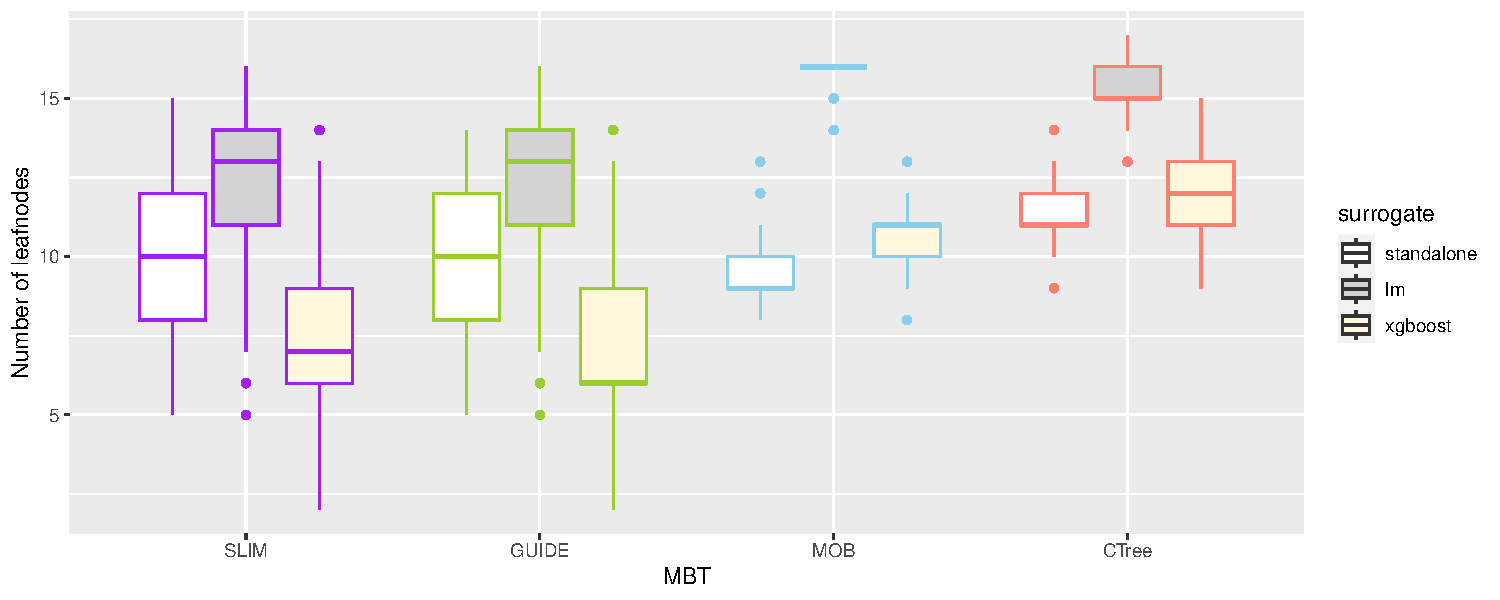
\includegraphics[width=11cm]{Figures/simulations/batchtools/basic_scenarios/linear_smooth/ls_1000_int.pdf}
\end{figure}  
\end{frame}


\begin{frame}{Linear Smooth - Performance}
\begin{figure}
\caption{Simulation results of stand alone MBTs on Scenario Linear Smooth with $n = 1000, alpha = 0.001, impr = 0.1$}
    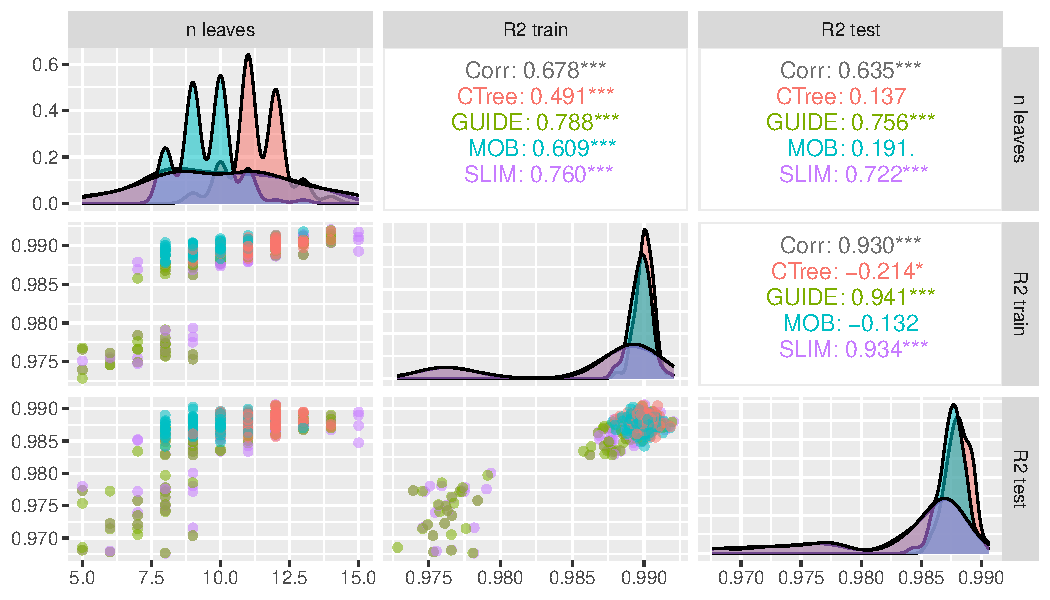
\includegraphics[width=11cm]{Figures/simulations/batchtools/basic_scenarios/linear_smooth/ls_1000_standalone_r2_nleaves.pdf}
\end{figure}   

    
\end{frame}

\begin{frame}{Linear Smooth - Performance}
\begin{figure}
    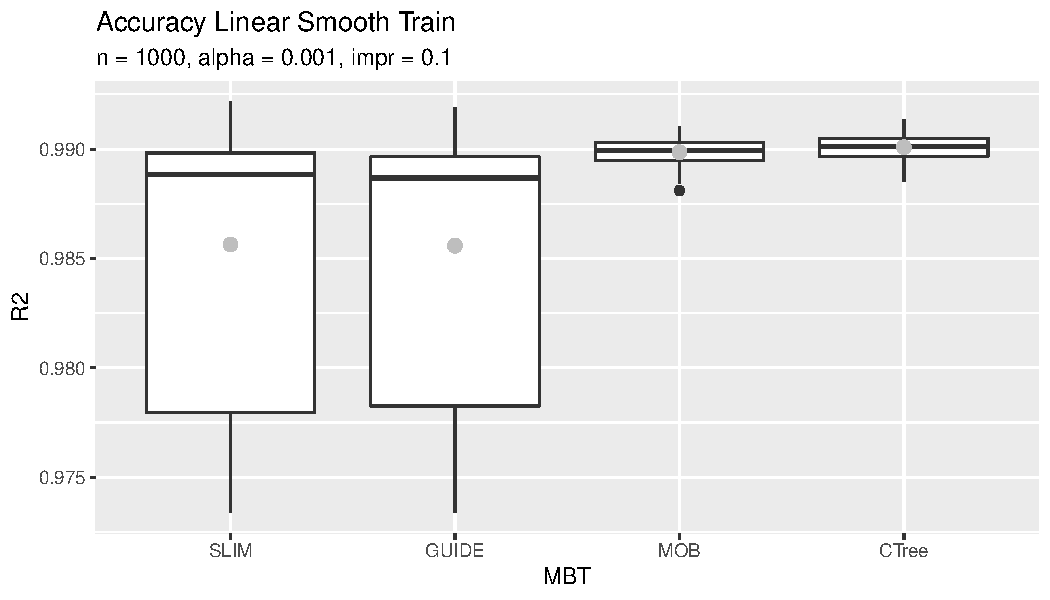
\includegraphics[width=11cm]{Figures/simulations/batchtools/basic_scenarios/linear_smooth/ls_1000_standalone_r2_train.pdf}
\end{figure}  
    
\end{frame}


\begin{frame}{Linear Smooth - Stability}
\begin{figure}
\caption{Stability simulation results of stand alone MBTs on Scenario Linear Smooth with $n = 1000, alpha = 0.001, impr = 0.1$. Only RI values for pairs with the same number of leaf nodes are considered.}
    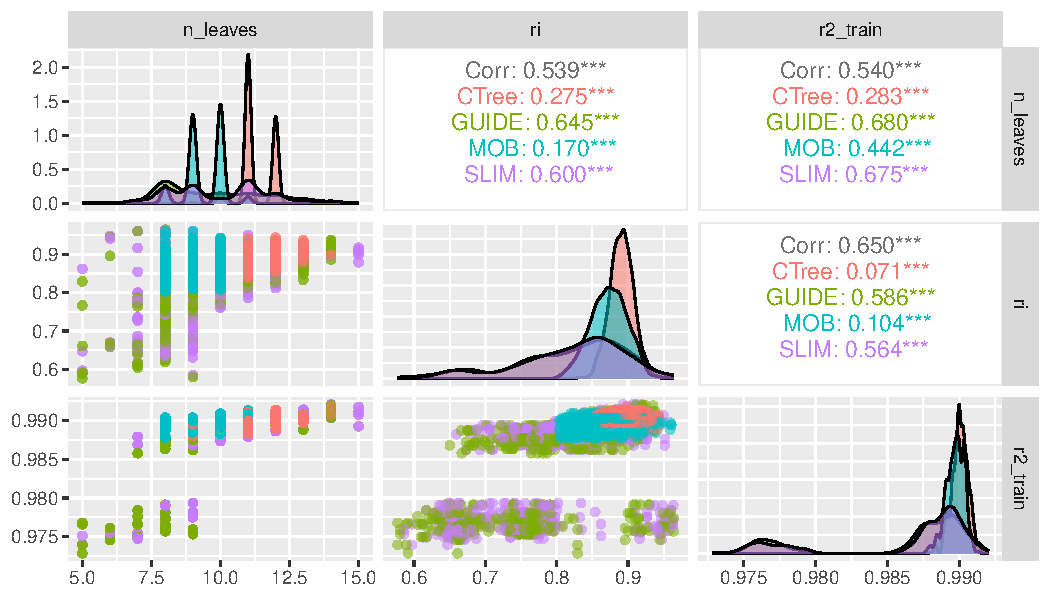
\includegraphics[width=11cm]{Figures/simulations/batchtools/basic_scenarios/linear_smooth/ls_1000_standalone_overview.pdf}
\end{figure}  
    
\end{frame}

\begin{frame}{Linear Smooth - Stability}
\begin{figure}
    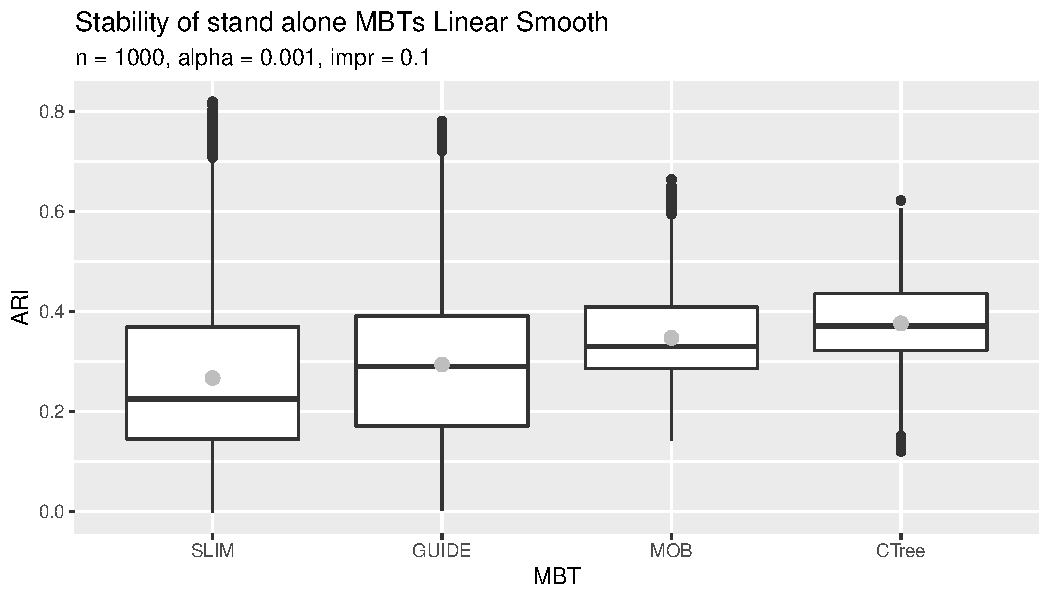
\includegraphics[width=11cm]{Figures/simulations/batchtools/basic_scenarios/linear_smooth/ls_1000_standalone_sta.pdf}
\end{figure}  
    
\end{frame}




\begin{frame}{Linear Smooth}
\textbf{Observations:}
\begin{itemize}
    \item All four algorithms achieve good performance
    \item The number of leaf nodes is high considering that the data generating process is very simple and involves only one interaction (increases even more with larger n)    
    \item SLIM and GUIDE are very sensitive regarding the choice of impr
    \item  given the number of leave nodes is identical, MOB and GUIDE provide more stable MBTs and have a better performance.

\end{itemize}

\textbf{Suggestion:}\\
Select a smaller maximum tree depth and a larger min node size in order to avoid large fluctuations and to obtain trees that are easier to interpret.

    
\end{frame}




\begin{frame}{Linear Abrupt}
\textbf{Data:}
\begin{itemize}
    \item $x_1, x_2 \sim U(-1,1)$, $x_3 \sim Bern(0.5)$
    \item $ f_{la}(x) = x_{1} - 8  x_2 + 16  x_2  \mathbf{I}_{x_3 = 0} + 8  x_2  \mathbf{I}_{x_1 > mean(x_1)}$
    \item $\epsilon \sim N(0, 0.1 sd(f_{la}(x))$
    \item $y = f_{la}(x) + \epsilon$
\end{itemize} 

\textbf{Settings:}
\begin{itemize}
    \item max tree depth = 7 
    \item min node size = 50    
\end{itemize}
\end{frame}


\begin{frame}{Linear Abrupt}
\textbf{Comparison of MBTs as stand alone models}
\begin{table}

\caption{Mean simulation results on 100 simulation runs for \textbf{SLIM} and \textbf{GUIDE}  as stand alone model on scenario Linear abrupt with $n = 1000$ for different values of $impr$}
\centering \tiny
\begin{tabular}[t]{r|r|r|r|r|r|r|r|r}
\hline
MBT & impr & mean n leaves & n leaves min & n leaves max & mean R2 train & sd R2 train & mean R2 test & sd R2 test\\
\hline
SLIM & 0.15 & 2.00 & 2 & 2 & 0.8272 & 0.0071 & 0.8250 & 0.0111\\
\hline
SLIM & 0.10 & 3.99 & 3 & 4 & 0.9884 & 0.0069 & 0.9870 & 0.0078\\
\hline
SLIM & 0.05 & 4.00 & 4 & 4 & 0.9891 & 0.0010 & 0.9878 & 0.0028\\
\hline
GUIDE & 0.15 & 2.00 & 2 & 2 & 0.8272 & 0.0071 & 0.8250 & 0.0111\\
\hline
GUIDE & 0.10 & 3.99 & 3 & 4 & 0.9884 & 0.0069 & 0.9870 & 0.0078\\
\hline
GUIDE & 0.05 & 4.00 & 4 & 4 & 0.9891 & 0.0010 & 0.9878 & 0.0028\\
\hline
\end{tabular}
\end{table}

\begin{table}
\caption{Mean simulation results on 100 simulation runs for \textbf{MOB} and \textbf{CTree}  as stand alone model on scenario Linear abrupt with $n = 1000$ for different values of $alpha$}
\centering \tiny
\begin{tabular}[t]{r|r|r|r|r|r|r|r|r}
\hline
MBT & alpha & mean n leaves & n leaves min & n leaves max & mean R2 train & sd R2 train & mean R2 test & sd R2 test\\
\hline
MOB & 0.001 & 12.77 & 10 & 15 & 0.9661 & 0.0083 & 0.9558 & 0.0091\\
\hline
MOB & 0.010 & 14.40 & 12 & 16 & 0.9736 & 0.0067 & 0.9641 & 0.0076\\
\hline
MOB & 0.050 & 14.85 & 13 & 17 & 0.9747 & 0.0063 & 0.9654 & 0.0071\\
\hline
CTree & 0.001 & 11.87 & 10 & 14 & 0.9484 & 0.0030 & 0.9390 & 0.0052\\
\hline
CTree & 0.010 & 12.82 & 11 & 15 & 0.9498 & 0.0030 & 0.9404 & 0.0051\\
\hline
CTree & 0.050 & 13.61 & 11 & 16 & 0.9508 & 0.0029 & 0.9411 & 0.0048\\
\hline
\end{tabular}
\end{table}

\end{frame}



\section{Linear Abrupt}
\begin{frame}{Linear Abrupt - Interpretability}

\begin{figure}
    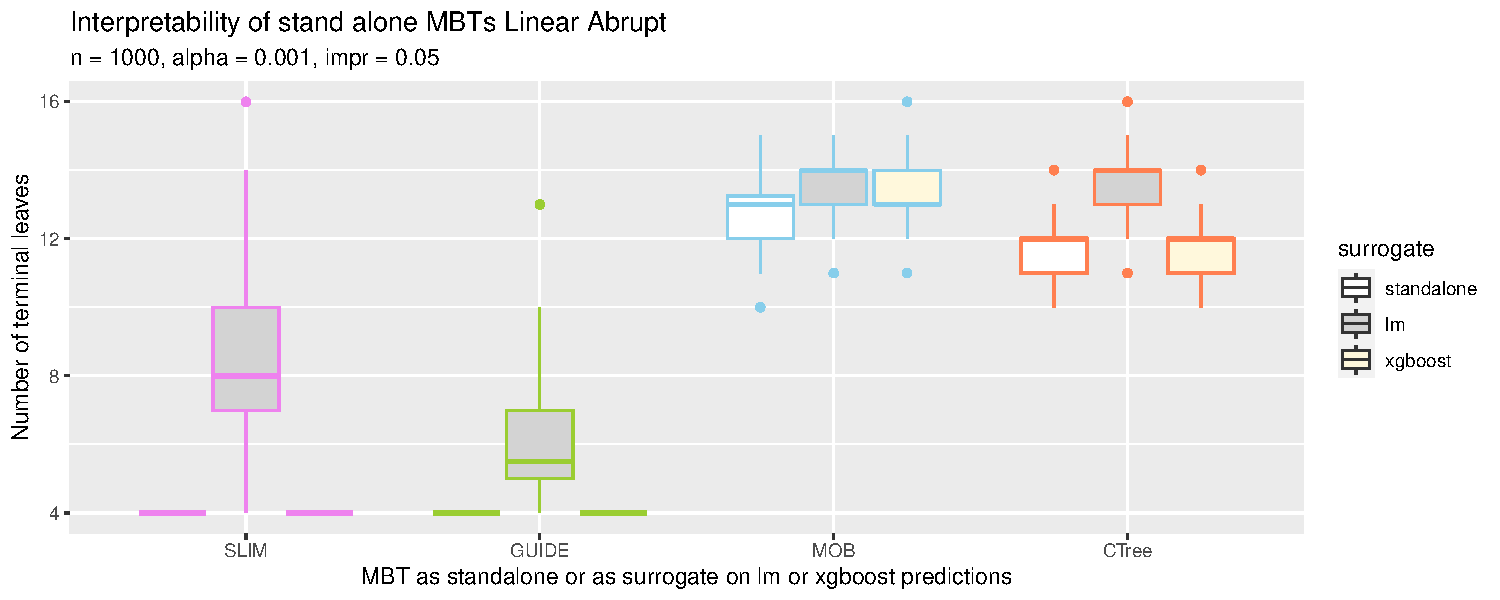
\includegraphics[width=11cm]{Figures/simulations/batchtools/basic_scenarios/linear_abrupt/la_1000_int.pdf}
\end{figure}    
\begin{itemize}
    \item Despite the small value for impr, SLIM and GUIDE generate only very small trees on the original data 
    \item When SLIM and GUIDE are used as surrogates for a linear model, the number of leaf nodes increases and varies strongly (more pronounced with SLIM than with guide). However, it remains below the number of leaf nodes for MOB and CTree.
\end{itemize}
\end{frame}


\begin{frame}{Linear Abrupt - Performance}
\begin{figure}
    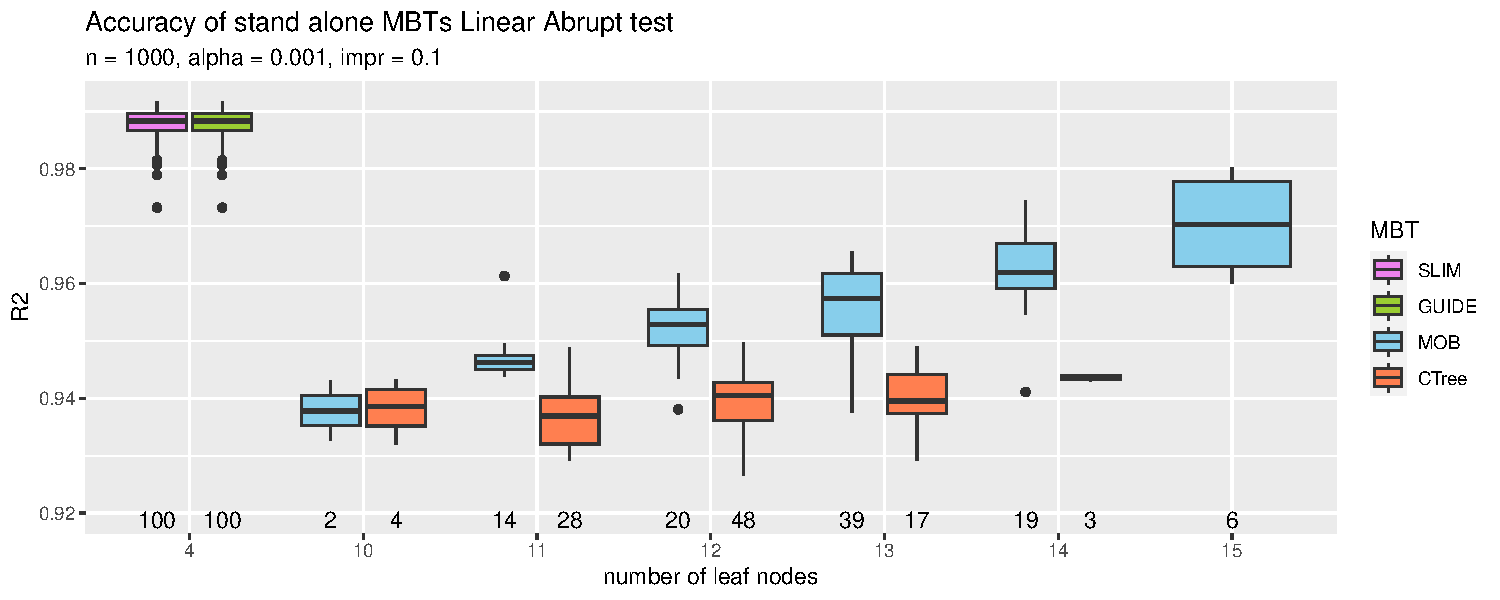
\includegraphics[width=11cm]{Figures/simulations/batchtools/basic_scenarios/linear_abrupt/la_1000_standalone_r2_test.pdf}
\end{figure}     
\begin{itemize}
    \item SLIM and GUIDE achieve better performance despite lower number of leaf nodes
    \item MOB has better performance than CTree (This could be due to the fact that abrupt splits are more difficult to detect with the linear test statistics in CTree \citep{Schlosser.2019})
\end{itemize}
\end{frame}

\begin{frame}{Linear Abrupt - Stability}
\begin{figure}
    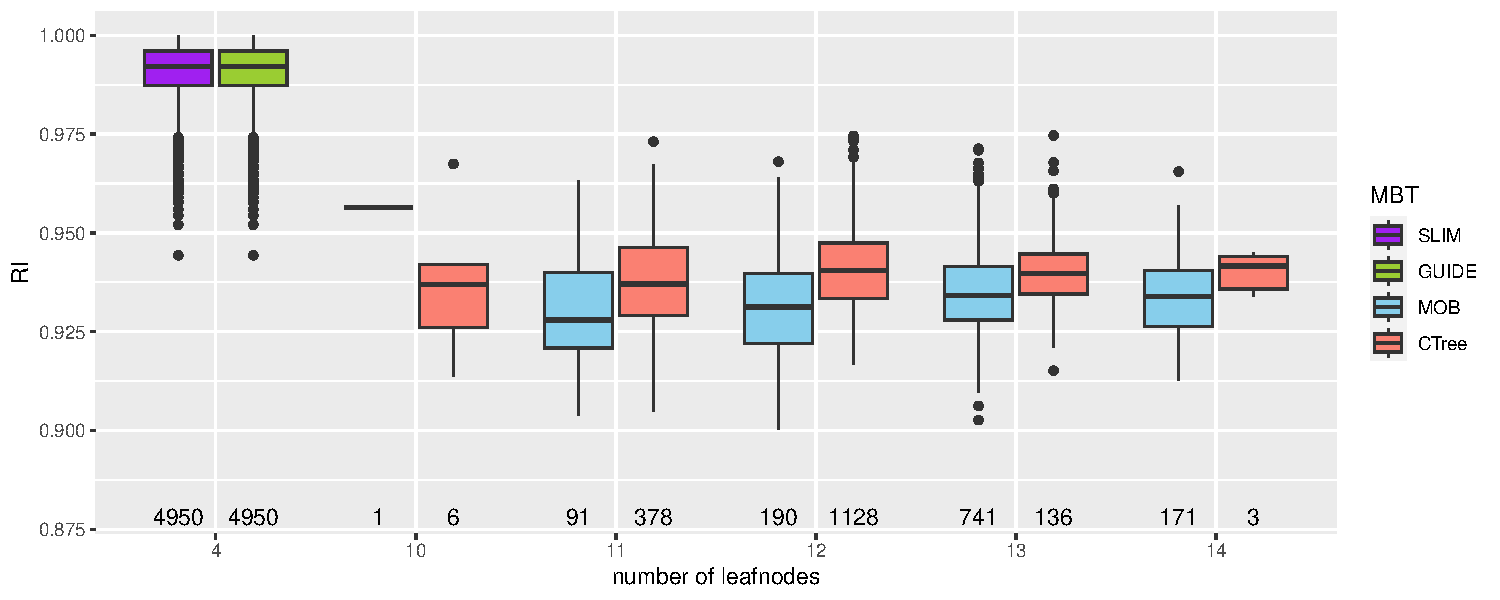
\includegraphics[width=11cm]{Figures/simulations/batchtools/basic_scenarios/linear_abrupt/la_1000_standalone_sta.pdf}
\end{figure}     
\end{frame}


\section{Linear Mixed}
\begin{frame}{Linear Mixed}
\textbf{Data}
\begin{itemize}
    \item $x_1,x_2 \sim U(-1,1)$  $x_3, x_4 \sim Bern(0.5)$
    \item $ f_{lm}(x) = 4 x_2 + 2 x_4 + 4 x_1 x_2 + 8 x_2 \mathbf{I}_{x_3 = 0} + 1 x_1 x_2 \mathbf{I}_{x_4 = 1}  $
    \item $\epsilon \sim N(0, 0.1 sd(f_{lm}(x))$
    \item $y = f_{lm}(x) + \epsilon$
\end{itemize}

\textbf{Settings:}
\begin{itemize}
    \item max tree depth = 7 
    \item min node size = 50    
\end{itemize}

\end{frame}   

\begin{frame}{Linear Mixed}
\begin{table}

\caption{Mean simulation results on 100 simulation runs for \textbf{SLIM} and \textbf{GUIDE}  as stand alone model on scenario Linear abrupt with $n = 1000$ for different values of $impr$}
\centering \tiny
\begin{tabular}[t]{r|r|r|r|r|r|r|r|r}
\hline
MBT & impr & mean n leaves & n leaves min & n leaves max & mean R2 train & sd R2 train & mean R2 test & sd R2 test\\
\hline
SLIM & 0.15 & 3.40 & 2 & 11 & 0.8853 & 0.0309 & 0.8771 & 0.0336\\
\hline
SLIM & 0.10 & 13.07 & 8 & 16 & 0.9801 & 0.0073 & 0.9743 & 0.0083\\
\hline
SLIM & 0.05 & 14.73 & 13 & 16 & 0.9830 & 0.0019 & 0.9774 & 0.0029\\
\hline
GUIDE & 0.15 & 3.29 & 2 & 11 & 0.8839 & 0.0305 & 0.8758 & 0.0329\\
\hline
GUIDE & 0.10 & 12.52 & 7 & 15 & 0.9789 & 0.0087 & 0.9732 & 0.0091\\
\hline
GUIDE & 0.05 & 14.19 & 12 & 16 & 0.9822 & 0.0024 & 0.9766 & 0.0032\\
\hline
\end{tabular}
\end{table}

\begin{table}

\caption{Mean simulation results on 100 simulation runs for \textbf{MOB} and \textbf{CTree}  as stand alone model on scenario Linear abrupt with $n = 1000$ for different values of $alpha$}
\centering \tiny
\begin{tabular}[t]{r|r|r|r|r|r|r|r|r}
\hline
MBT & alpha & mean n leaves & n leaves min & n leaves max & mean R2 train & sd R2 train & mean R2 test & sd R2 test\\
\hline
MOB & 0.15 & 14.52 & 13 & 17 & 0.9802 & 0.0017 & 0.9725 & 0.0027\\
\hline
MOB & 0.10 & 14.73 & 13 & 17 & 0.9803 & 0.0017 & 0.9726 & 0.0028\\
\hline
MOB & 0.05 & 14.80 & 13 & 17 & 0.9804 & 0.0017 & 0.9727 & 0.0028\\
\hline
CTree & 0.15 & 14.80 & 12 & 17 & 0.9802 & 0.0017 & 0.9731 & 0.0023\\
\hline
CTree & 0.10 & 14.98 & 13 & 17 & 0.9802 & 0.0017 & 0.9731 & 0.0023\\
\hline
CTree & 0.05 & 15.03 & 13 & 17 & 0.9802 & 0.0017 & 0.9731 & 0.0023\\
\hline
\end{tabular}
\end{table}
    
\end{frame}



\begin{frame}{Linear Mixed - Interpretability}
For  $alpha= 0.001$ and $impr = 0.05$ the mean number of leaf nodes nodes is similar for the four MBT Algorithms
\begin{figure}
    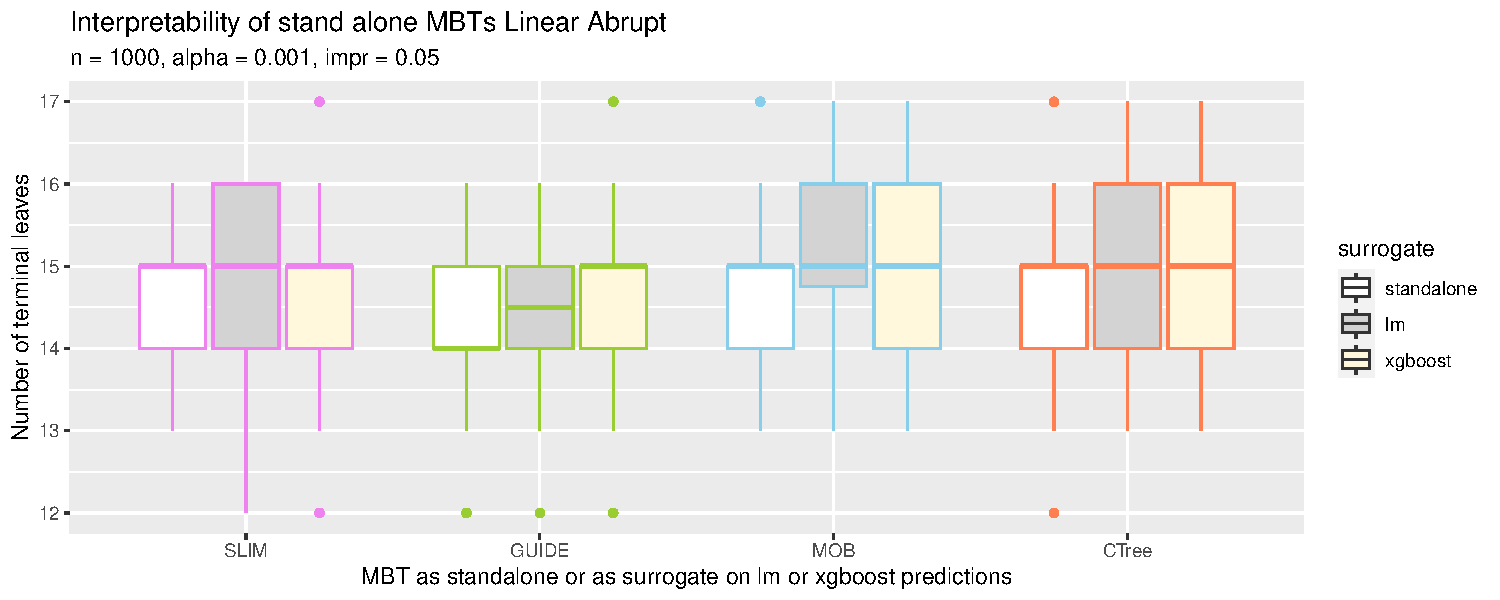
\includegraphics[width=11cm]{Figures/simulations/batchtools/basic_scenarios/linear_mixed/lm_1000_int.pdf}
\end{figure}     
\end{frame}

\begin{frame}{Linear Mixed - Performance}

\begin{figure}
    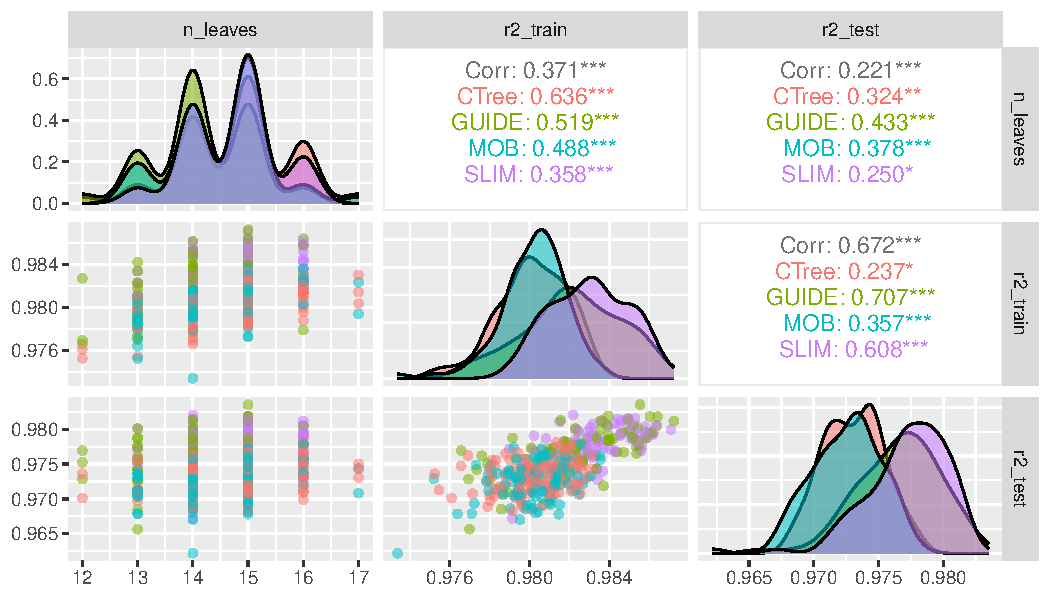
\includegraphics[width=11cm]{Figures/simulations/batchtools/basic_scenarios/linear_mixed/lm_1000_standalone_r2_nleaves.pdf}
\end{figure}  
\end{frame}

\begin{frame}{Linear Mixed - Performance}

\begin{figure}
    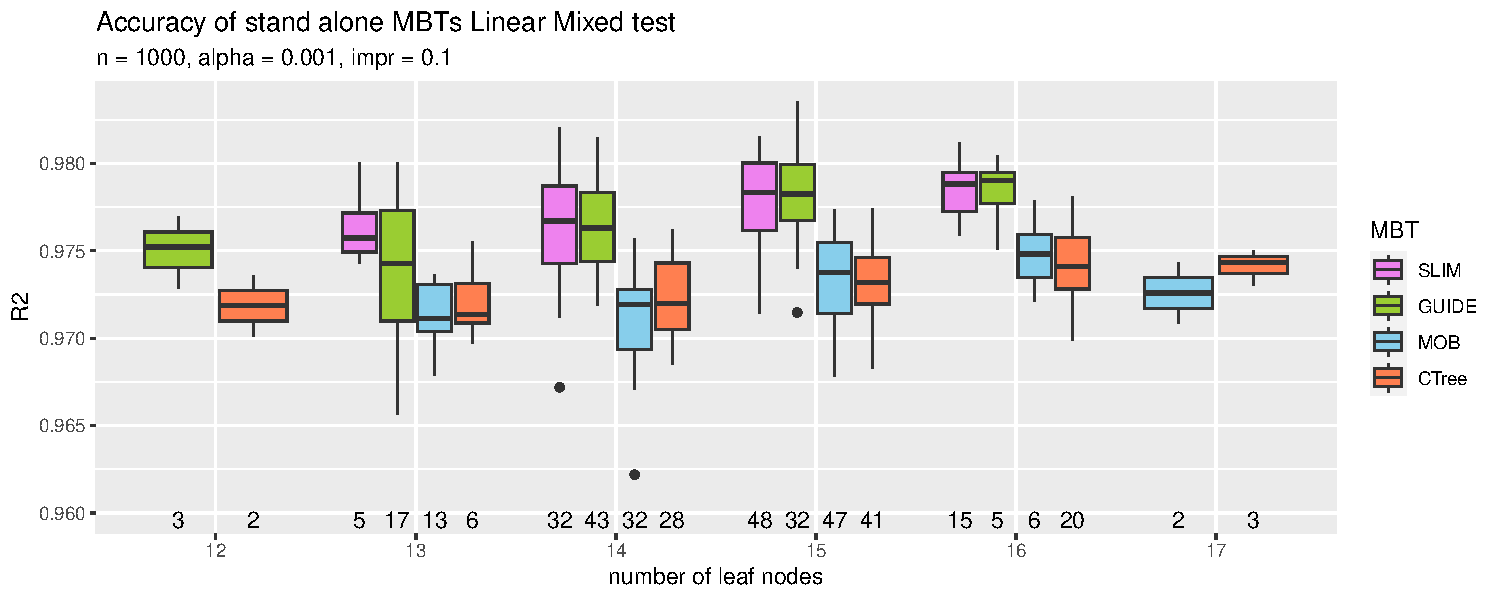
\includegraphics[width=11cm]{Figures/simulations/batchtools/basic_scenarios/linear_mixed/lm_1000_standalone_r2_test.pdf}
\end{figure}  
\end{frame}


\begin{frame}{Linear Mixed - Stability}

\begin{figure}
    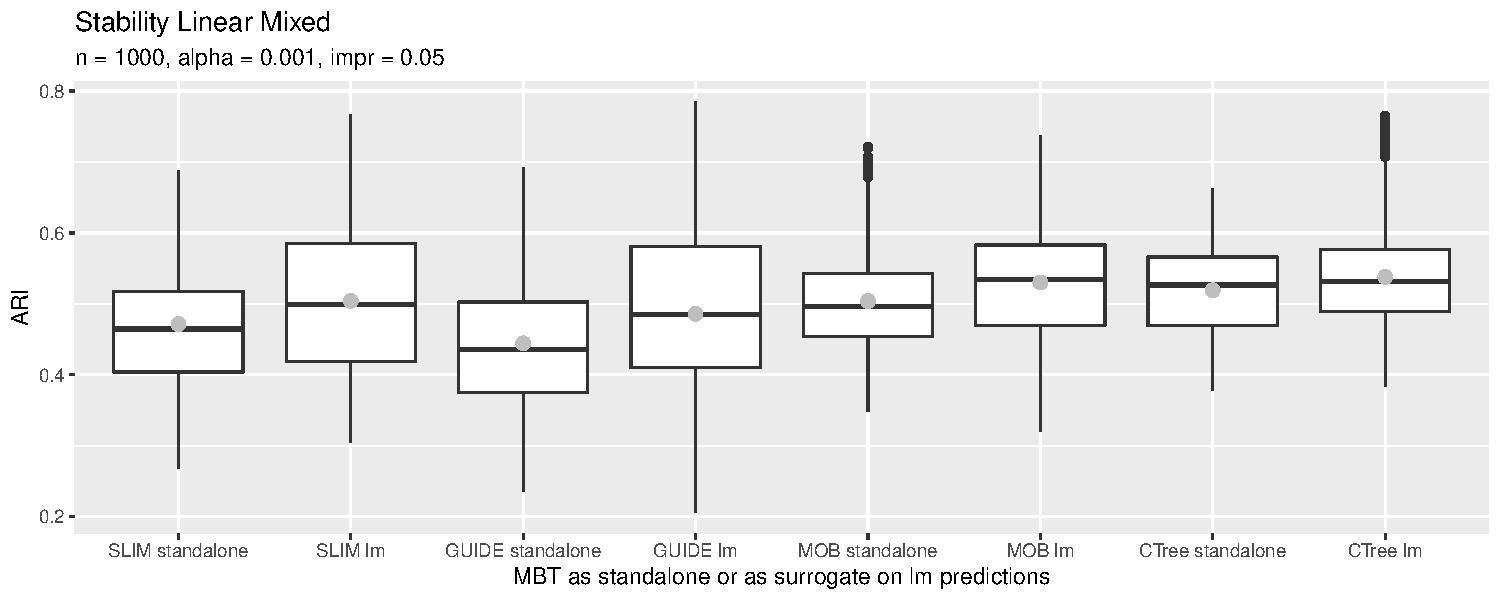
\includegraphics[width=11cm]{Figures/simulations/batchtools/basic_scenarios/linear_mixed/lm_1000_standalone_lm_sta.pdf}
\end{figure}     
\begin{itemize}
    \item Here stability is almost everywhere higher if the MBTs are used as surrogates (as stated in the SLIM Paper)
\end{itemize}

\end{frame}


\section{Correlated Data}
\begin{frame}{Correlated Data}
\textbf{Data}
\begin{itemize}
    \item $x_1,..., x_3 \sim U(-1,1), cor(x_1,x_2) = \rho_{12} \in \{0.1, 0.5, 0.9\}$ 
    \item $ f_{ls}(x) = x_1 + 4   x_2 + 3   x_2   x_3 $
    \item $\epsilon \sim N(0, 0.1 sd(f_{ls}(x))$
    \item $y = f_{ls}(x) + \epsilon$
\end{itemize}

\textbf{Question:} \\
Are there differences between the algorithms when correlated data are included? How often is $x_1$ incorrectly chosen as a splitting variable?
    
\end{frame}

\begin{frame}{Correlated Data}
\begin{table}

\caption{Mean simulation results, in particular, the relative frequency that x1 was chosen as a splitting variable by an MBT algorithm, on 500 simulation runs as stand alone model on scenario Correlated Data with n = 1000, alpha = 0.001, impr = 0.01}
\centering
\begin{tabular}[t]{l|r|r|r|r|r}
\hline
MBT & rho & frequency of x1  & number of leaf nodes & R2 train & R2 test\\
\hline
SLIM & 0.1 & 0.096 & 10.140 & 0.9860 & 0.9832\\
\hline
GUIDE & 0.1 & 0.058 & 9.950 & 0.9859 & 0.9832\\
\hline
MOB & 0.1 & 0.000 & 9.386 & 0.9898 & 0.9876\\
\hline
CTree & 0.1 & 0.000 & 11.294 & 0.9901 & 0.9881\\
\hline
SLIM & 0.5 & 0.144 & 9.892 & 0.9865 & 0.9839\\
\hline
GUIDE & 0.5 & 0.126 & 9.654 & 0.9864 & 0.9840\\
\hline
MOB & 0.5 & 0.000 & 9.034 & 0.9899 & 0.9878\\
\hline
CTree & 0.5 & 0.000 & 10.682 & 0.9900 & 0.9882\\
\hline
SLIM & 0.9 & 0.322 & 9.826 & 0.9866 & 0.9842\\
\hline
GUIDE & 0.9 & 0.384 & 9.784 & 0.9870 & 0.9848\\
\hline
MOB & 0.9 & 0.058 & 8.690 & 0.9899 & 0.9879\\
\hline
CTree & 0.9 & 0.036 & 10.216 & 0.9900 & 0.9883\\
\hline
\end{tabular}
\end{table}    
\end{frame}


\begin{frame}{Bibliography}
    \bibliography{bibliography}
    \bibliographystyle{dcu}

\end{frame}
\end{document}